
%----------------------------------------------------------------------------------------
%	CHAPTER 2
%----------------------------------------------------------------------------------------
\chapterimage{chapter_head_2.pdf} % Chapter heading image

\chapter{Treinando o \bodycontrol}
\label{chap:trainingbodycontrol}

\begin{comment}
\index{Neurociência}
\begin{definition}[Neurociência] Seguindo o dicionario médico Merriam-Webster \cite{merriamwebster-neuroscience} 
a neurociência é a ciência que se encarrega do estudo da anatomia, fisiologia, 
bioquímica ou biologia molecular dos nervos e o tecido nervoso e, especialmente, sua relação com o comportamento e a aprendizagem.

Sobre as áreas de estudo, Roberto Lent no seu livro ``Cem bilhões de neurônios - Conceitos fundamentais de neurociência''
\cite[pp. 6]{lent2004cem}
classifica a diversidade das metodologias da neurociência nos seguintes tópicos:
\begin{itemize}
\item neurociência molecular (neuroquímica ou neurobiologia molecular), 
\item neurociência celular (neurocitologia ou neurobiologia celular),
\item neurociência sistêmica (inclui a Neuro-histologia ou neuroanatomia, neurofisiologia), 
\item neurociência comportamental e
\item neurociência cognitiva (neuropsicologia).
\end{itemize}
\end{definition}

\index{Neurociência cognitiva}
\begin{definition}[Neurociência cognitiva] 
É o campo da ciência com foco no estudo dos substratos neurais dos processos mentais como a linguagem, a autoconsciência, a memória, entre outras \cite[pp. 6]{lent2004cem} \cite{NatureCognitiveNeuroscience}.
Este campo de estudo é a intersecção da psicologia e da neurociência, porém também se sobrepõe à psicologia fisiológica, psicologia cognitiva e neuropsicologia. 
Assim a neurociência cognitiva combina as teorias da psicologia cognitiva e modelagem computacional com dados experimentais sobre o cérebro  \cite{NatureCognitiveNeuroscience}.
\end{definition}
\end{comment}

Como foi visto na Seção \ref{subsec:sec-motor-cognitive-multicomponente},
o \hyperref[subsec:sec-motor-cognitive-multicomponente]{\textbf{treinamento cognitivo-motor multicomponente}}
tem se demostrado como uma ferramente eficiente para o incremento da cognição.
Consequentemente, um treinamento de dança que trabalhe com múltiplos componentes
%como: 
%escutar e seguir um ritmo ou melodia na música, 
%realizar um movimento com nosso corpo,
%pensar na posição de um objeto externo a nós (ex: nosso par de dança);
pode ser utilizado para fixar as funções cognitivas necessárias para dançar 
de forma fluente e sem estresse físico ou mental.

%http://www.folha1.com.br/_conteudo/2012/04/blogs/sermotriz/1118441-treinamento-cognitivo-melhora-do-processamento-mental-em-busca-de-performance.html
%https://sbgg.org.br/publicacoes-cientificas/sbgg-atual/sbgg-artigos-n-17/beneficios-do-treino-cognitivo/


%%%%%%%%%%%%%%%%%%%%%%%%%%%%%%%%%%%%%%%%%%%%%%%%%%%%%%%%%%%%%%%%%%%%%%%%%%%%%%%%
%%%%%%%%%%%%%%%%%%%%%%%%%%%%%%%%%%%%%%%%%%%%%%%%%%%%%%%%%%%%%%%%%%%%%%%%%%%%%%%%
\section{Exemplos de treinamentos cognitivo-motor multicomponente}

Os exemplos presentados a continuação trabalham três componentes necessários na dança,
estes são:
\begin{itemize}
\item A \hyperref[cap:percepcaomusical]{\textbf{percepção musical}}: 
neste caso serão trabalhadas a \hyperref[sec:percepcionmetrica]{\textbf{percepção da métrica}} 
e/ou \hyperref[sec:perceberfrases]{\textbf{das frases musicais}}, 
as quais podem ser extraídas de uma música ou de algum ritmo simples gerado digitalmente.
\item O \hyperref[sec:BodyControl]{\textbf{controle corporal}}: 
no qual executaremos um movimento ou passo de dança que estará subordinado
à métrica escolhida no item anterior.
\item A atividade externa: representada por um objeto ou atividade
as quais devemos comandar ou conduzir seguindo a métrica escolhida.
\end{itemize}

\begin{example}[Treino cognitivo-motor multicomponente com movimentos simples:]
\label{ex:treino-cognitivo-multi-simples}
Como é mostrado na Tabela \ref{tab:treino-bolinha1}, 
neste exercício devemos escolher trés componentes distintos os quais executaremos de forma simultânea.
\begin{itemize}
\item A primeira escolha corresponde ao ritmo que seguiremos em nosso treinamento, 
este pode ser 
um ``tchic tchic tum'', \meter{2}{4}\leftrepeat~\Vier\Acht\Acht~\rightrepeat, ou 
um ``tum tum'', \meter{2}{4}\leftrepeat~\Vier\Vier~\rightrepeat, 
em qualquer destes dois casos um ``tum'' deve coincidir com o \hyperref[subsec:perceberTF1]{\textbf{tempo forte}}.
A fonte de informação musical pode vir de
    \begin{itemize}
    \item uma música em compasso binário, ex: ``Suingue de Samba'' interpretado por Rogê (ritmo 2), ou de 
    \item um metrônomo (ritmo 1).
    \end{itemize}
Neste caso o importante é souber \hyperref[subsec:perceberTF1]{\textbf{reconhecer o tempo forte}}.
\item A segunda escolha corresponde ao movimento a ser realizado, os quais podem ser:
    \begin{itemize}
    \item caminhadas ou balanços se o ritmo escolhido é ``tum tum'', e
    \item caminhadas, básicos frente trás ou cruzados se nosso ritmo escolhido é um ``tchic tchic tum''.
    \end{itemize}
Em ambos casos realizaremos uma pisada com troca de peso do corpo por cada figura musical.
\item A terceira escolha é a atividade externa, a qual podem ser: 
    \begin{itemize}
    \item jogar uma bolinha ao ar e pegar-lha novamente exatamente quando se escute o tempo forte (atividade 1), ou podemos 
    \item jogar uma bolinha ao chão de modo que esta rebote no exato momento em que se escute o tempo forte (atividade 2).
    \end{itemize}
\end{itemize}
\end{example}

\begin{table}[!h]
  \centering
    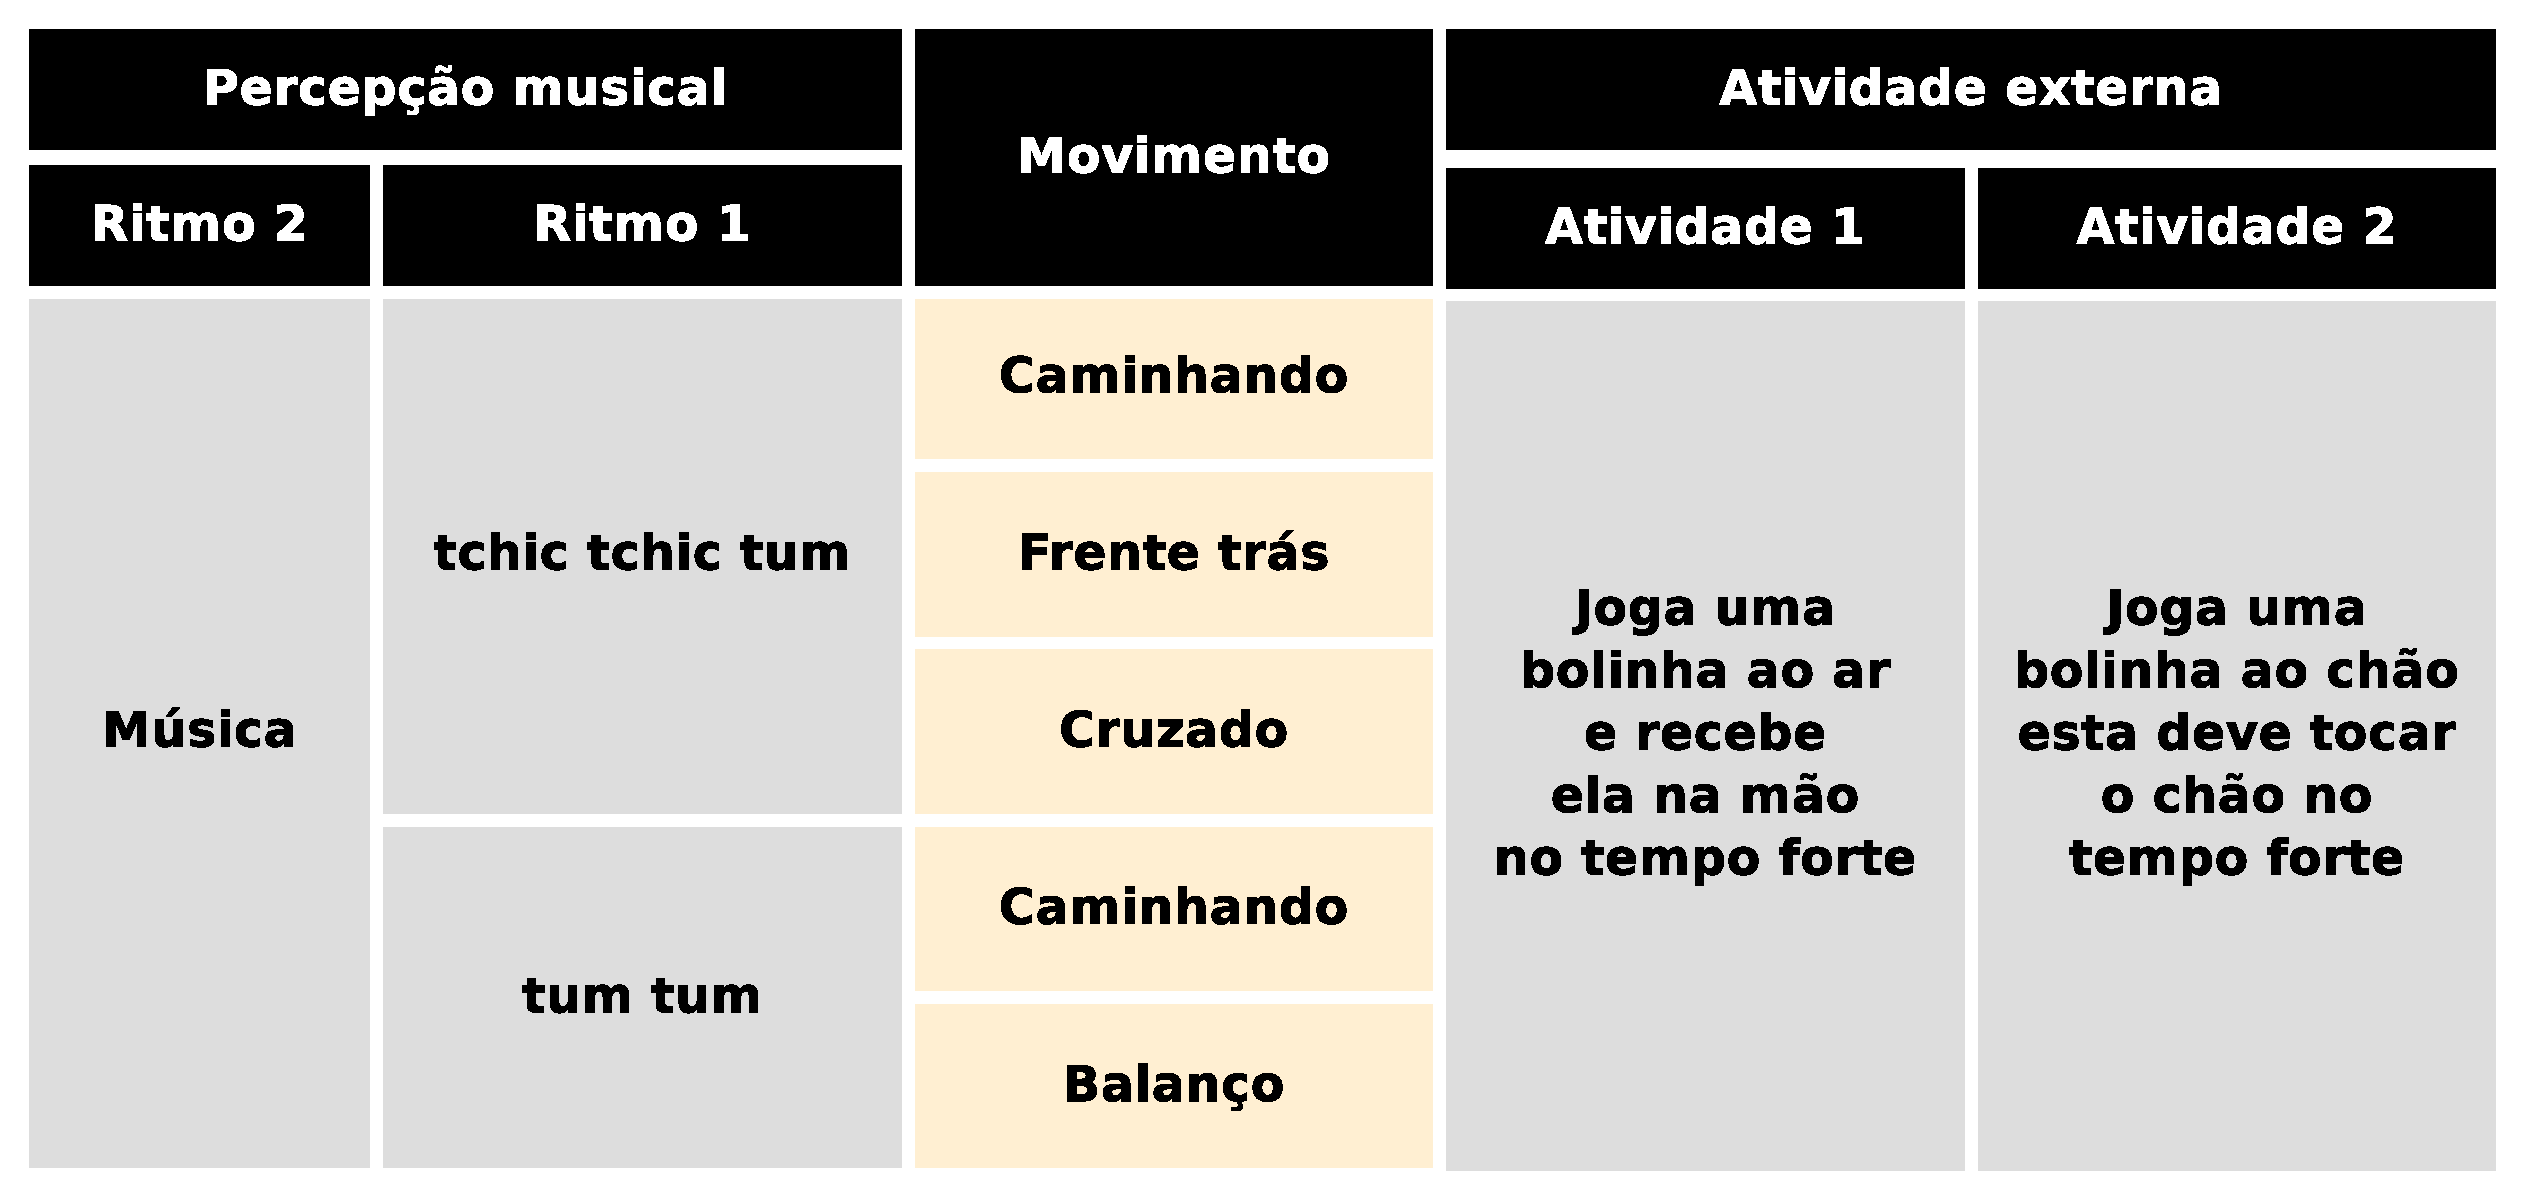
\includegraphics[width=1.0\textwidth]{chapters/cap-body-control/treino-bolinha1.eps}
\caption{Treino cognitivo-motor multicomponente com movimentos simples.}
\label{tab:treino-bolinha1}
\end{table}


Se o Exemplo \ref{ex:treino-cognitivo-multi-simples} resulta simples de seguir, 
pode ser interessante pausar aleatoriamente no meio da música e 
aprender a voltar corretamente na métrica,
até que consigamos \hyperref[subsec:perceberTF1]{\textbf{reconhecer de forma fácil o tempo forte}}.
Com essas pausas evitamos que nosso cérebro crie um atalho,
e só identifique o tempo forte do primeiro compasso, e 
logo só conte os segundos até o próximo tempo forte.
%A ideia do exercício é ganhar a habilidade de voltar a pegar facilmente a 
%métrica da música após algum erro ou pausa na dança.



\begin{example}[Treino cognitivo-motor multicomponente com movimentos complexos:]
Este exemplo é similar ao Exemplo \ref{ex:treino-cognitivo-multi-simples}
no qual são trabalhadas em simultâneo trés componentes da dança,
com a diferença de que aqui só é usado o ritmo ``tchic tchic tum'', 
\meter{2}{4}\leftrepeat~\Vier\Acht\Acht~\rightrepeat,
o qual pode vir de: 
    \begin{itemize}
    \item uma música em compasso binário, ex: ``Piston de Gafieira'' interpretado por Toquinho (ritmo 2), ou de 
    \item um metrônomo (ritmo 1).
    \end{itemize}
Como mostra a Tabela \ref{tab:treino-bolinha2}, 
os movimentos que podemos escolher são um pouco mais complexos,
tais como a trança, escovinha, etc. 
e devem ser executados mediante uma troca de peso do corpo por cada figura musical.
Finalmente, as possíveis atividades externas são as mesmas que no 
Exemplo \ref{ex:treino-cognitivo-multi-simples}
\end{example}

\begin{table}[!h]
  \centering
    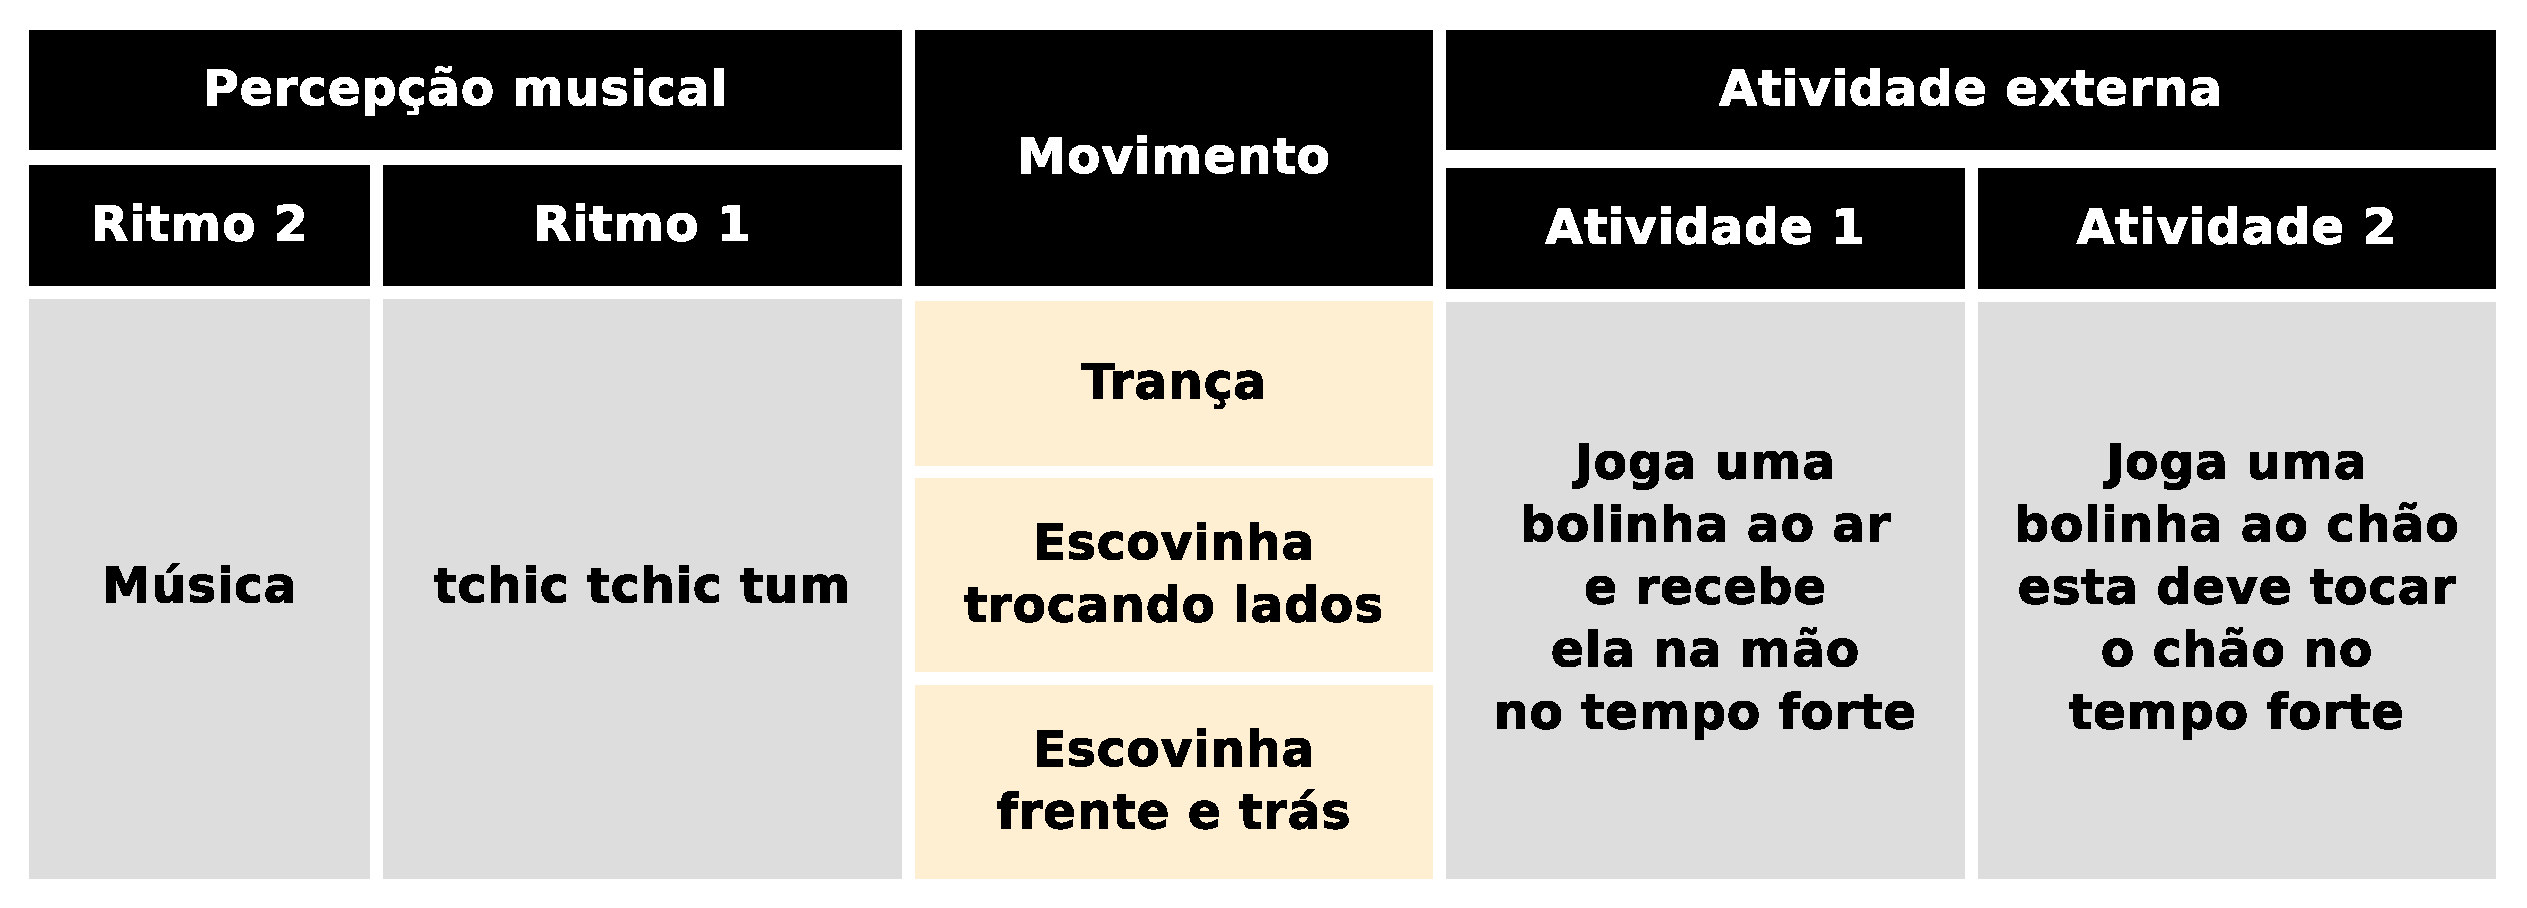
\includegraphics[width=1.0\textwidth]{chapters/cap-body-control/treino-bolinha2.eps}
\caption{Treino cognitivo-motor multicomponente com movimentos complexos.}
\label{tab:treino-bolinha2}
\end{table}

A seguir são mostrados alguns exemplos de treino cognitivo-motor multicomponente 
que ajudaram a explorar nosso controle corporal e a percepção das frases na música.

\begin{example}[Treino cognitivo-motor multicomponente relativo à percepção do final de frase musical:]
Como é mostrado na Tabela \ref{tab:treino-bolinha3},
neste exercício devemos escolher trés componentes distintas que serão executadas de forma simultânea.
\begin{itemize}
\item Na primeira escolha temos a percepção musical do 
\hyperref[pos:detetandoiniciofrase]{\textbf{final de frase musical}} 
e do último tempo forte da frase, na qual a fonte de informação musical pode vir de:
    \begin{itemize}
    \item uma música em compasso binário, ex: ``Cabide'' interpretado por Ana Carolina e Luiz Melodia (ritmo 2), ou
    \item um ritmo gerado de forma sintética (ritmo 1),
    ex: a melodia ``lamento e consolo'' mostrada na Figura \ref{fig:lamento-e-consolo}, 
    na qual todas as frases musicais finalizam no tempo forte.
    \end{itemize}
Neste caso o objetivo é usar uma música que nos permita treinar
como \hyperref[pos:detetandoiniciofrase]{\textbf{reconhecer o final de frase musical}}. 
É importante lembrar que as frases musicais podem ter um 
\hyperref[subsec:finaldefrasemus1]{\textbf{final masculino ou feminino}}, 
porém nos estamos interessados em reconhecer o ultimo tempo forte.
\item A segunda escolha corresponde ao movimento a ser realizado,
neste caso podemos usar:
    \begin{itemize}
    \item caminhadas ou balanços seguindo um ritmo ``tum tum'', 
    \meter{2}{4}\leftrepeat~\Vier\Vier~\rightrepeat, ou 
    \item caminhadas, básicos frente trás ou cruzados seguindo um ritmo ``tchic tchic tum'', 
    \meter{2}{4}\leftrepeat~\Vier\Acht\Acht~\rightrepeat.
    \end{itemize}
Em ambos casos realizaremos uma pisada com troca de peso do corpo por cada figura musical.
\item A terceira escolha é a atividade externa, as quais podem ser: 
    \begin{itemize}
    \item jogar uma bolinha ao ar e pegar-lha novamente exatamente no último tempo forte da cada frase musical (atividade 1), ou
    \item podemos jogar a bolinha ao chão de modo que rebote no último tempo forte da cada frase musical (atividade 2).
    \end{itemize}
\end{itemize}
\end{example}

\begin{table}[!h]
  \centering
    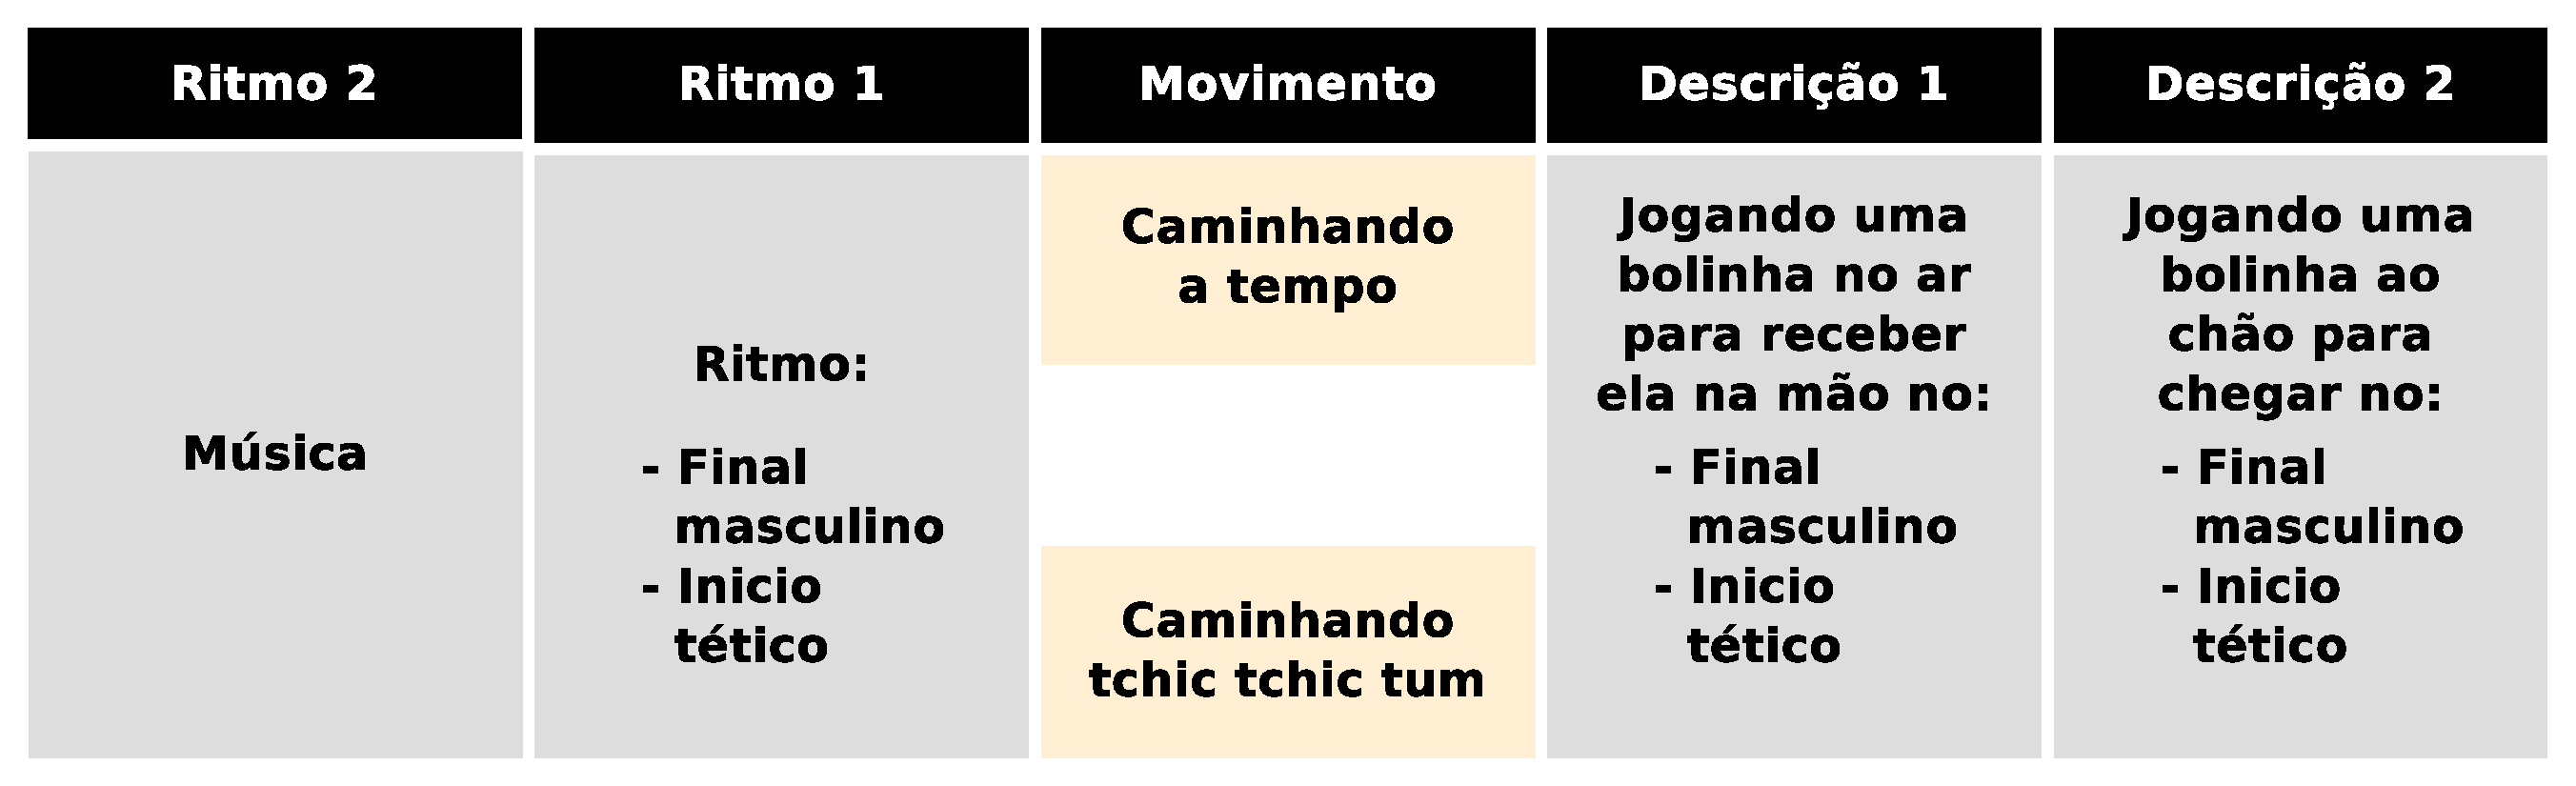
\includegraphics[width=1.0\textwidth]{chapters/cap-body-control/treino-bolinha3.eps}
\caption{Treino cognitivo-motor multicomponente relativo à percepção do final de frase musical.}
\label{tab:treino-bolinha3}
\end{table}



\begin{example}[Treino cognitivo-motor multicomponente relativo à percepção do inicio da frase musical:]
Como é mostrado na Tabela \ref{tab:treino-bolinha4},
neste exercício devemos escolher trés componentes que executaremos em simultâneo.
\begin{itemize}
\item A primeira escolha corresponde à percepção do \hyperref[pos:detetandoiniciofrase]{\textbf{inicio da frase musical}},
especificamente procuramos reconhecer o primeiro tempo forte da frase.
A fonte de informação musical pode vir de:
    \begin{itemize}
    \item uma música em compasso binário, ex: ``Tamborim'' interpretado pelo Clube do Balanço (ritmo 2) 
    o qual tem frases de 4 compassos fáceis de identificar, ou de
    \item um ritmo gerado de forma sintética (ritmo 1),
    ex: a melodia ``lamento e consolo'' mostrada na Figura \ref{fig:lamento-e-consolo}, 
    na qual todas as frases musicais tem um \hyperref[subsec:InicioFraseMusical]{\textbf{ritmo anacrústico}}
    fácil de acompanhar.
    \end{itemize}
Neste caso o importante é escolher uma música que nos permita treinar
como \hyperref[pos:detetandoiniciofrase]{\textbf{reconhecer o inicio da frase musical}}
e o primeiro tempo forte da frase. 
É importante lembrar que as frases musicais podem ter um inicio com 
\hyperref[subsec:InicioFraseMusical]{\textbf{ritmo tético, anacrústico ou acéfalo}}.
\item A segunda escolha que devemos fazer é o movimento a ser realizado,
neste caso podemos usar:
    \begin{itemize}
    \item caminhadas ou balanços em tempo, quer dizer seguindo um ritmo ``tum tum'', 
    \meter{2}{4}\leftrepeat~\Vier\Vier~\rightrepeat, e
    \item caminhadas, básicos frente trás ou cruzados seguindo um ritmo ``tchic tchic tum'', 
    \meter{2}{4}\leftrepeat~\Vier\Acht\Acht~\rightrepeat.
    \end{itemize}
Em ambos casos realizaremos uma pisada com troca de peso por cada figura musical.
\item A terceira escolha é a atividade externa, a qual pode ser: 
    \begin{itemize}
    \item mudar a direção de nosso movimento no primeiro tempo forte de cada frase musical (atividade 1), ou
    \item podemos jogar a bolinha ao chão de modo que rebote no último tempo forte da cada frase musical (atividade 2).
    \end{itemize}
\end{itemize}
\end{example}

\begin{table}[!h]
  \centering
    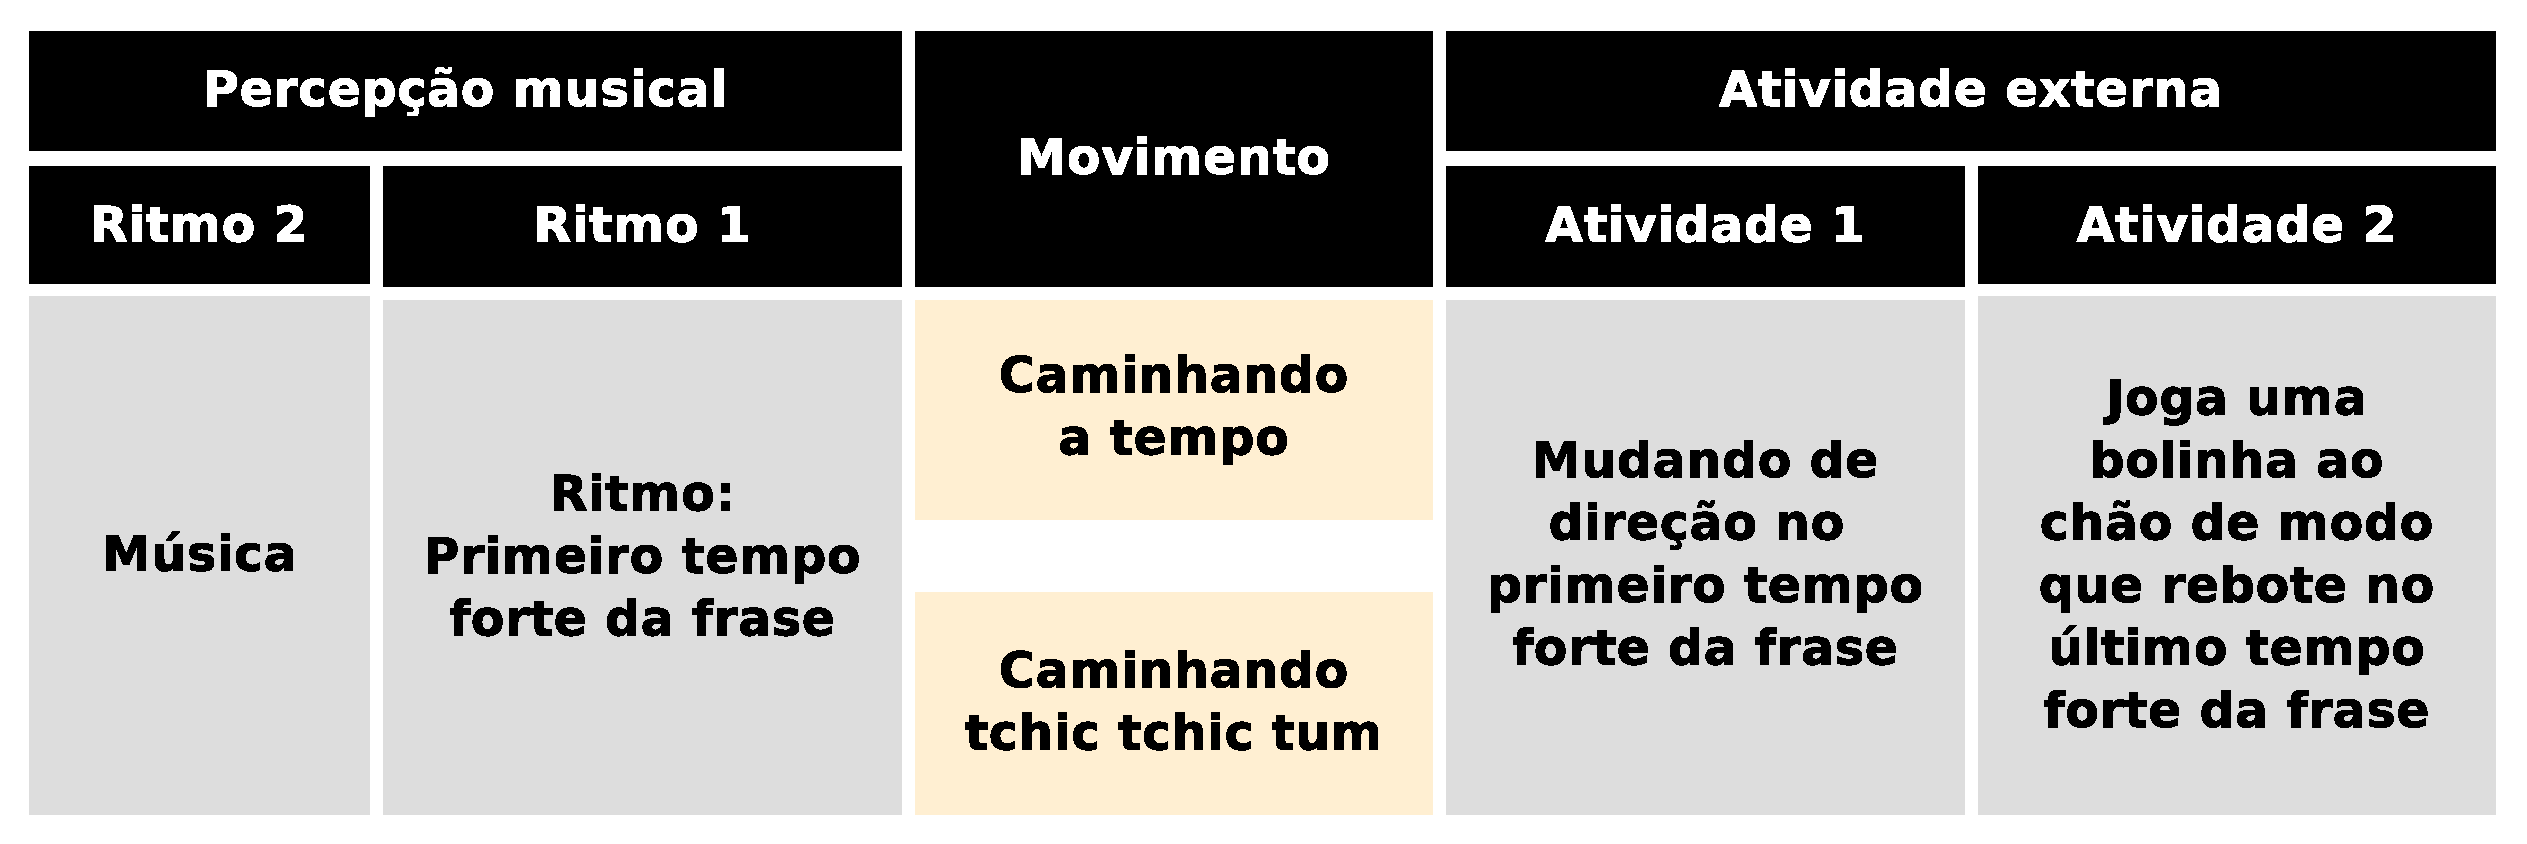
\includegraphics[width=1.0\textwidth]{chapters/cap-body-control/treino-bolinha4.eps}
\caption{Treino cognitivo-motor multicomponente relativo à percepção do inicio da frase musical.}
\label{tab:treino-bolinha4}
\end{table}


%\section{\textcolor{red}{  Treino de ombros no plano frontal}}
%\section{\textcolor{red}{  Treino do quadril no plano frontal}}



\section{Problemas no controle corporal}

%%%%%%%%%%%%%%%%%%%%%%%%%%%%%%%%%%%%%%%%%%%%%%%%%%%%%%%%%%%%%%%%%%%%%%%%%%%%%%%%
%%%%%%%%%%%%%%%%%%%%%%%%%%%%%%%%%%%%%%%%%%%%%%%%%%%%%%%%%%%%%%%%%%%%%%%%%%%%%%%%
%%%%%%%%%%%%%%%%%%%%%%%%%%%%%%%%%%%%%%%%%%%%%%%%%%%%%%%%%%%%%%%%%%%%%%%%%%%%%%%%
\subsection{Dançar saltitando}
\index{Problemas!Saltitar}

\begin{problemT}[Saltitar quando dançamos:]
Eu percebo que o saltitar na dança das pessoas pode ter em alguns casos um origem mental e em outros um origem físico.
\begin{itemize}
\item \textbf{Mental:} Algumas vesses, o saltitar
é o jeito que  uma pessoa tem para conseguir acompanhar o pulso ou a métrica da música. 
Isto, quando a pessoa ainda não entende esses conceitos de forma conscientemente
e só percebe que quando saltita consegue acompanhar melhor a música.
\item \textbf{Físico:} Outras vezes o saltitar na dança pode ser devido a que a pessoa se movimenta na dança
com o peso do corpo dividido em ambos pés, de modo que quando deseja movimentar algum deles,
a pessoa tem muita dificuldade de tirar esse pé do chão; 
pois sem importar qual escolha na movimentação, a pessoa perderá o equilíbrio,
pelo que para movimentar-se o dançarino desenvolve o saltitar; quer dizer, 
ele faz um efeito mola nos joelhos ao igual que os dançarinos de ``swing'', 
para que no momento que estiquem os joelhos a pessoa tenha uma oportunidade de movimentar algum pé.    
\end{itemize}
\end{problemT}


\begin{SolutionT}[Relativa ao problema de saltitar:]
Para solucionar o saltitar na nossa dança devemos nos perguntar se o origem é mental, físico ou ambos;
neste sentido podemos ter em conta as seguintes recomendações:
\begin{itemize}
\item  Aprender a reconhecer os tempos fortes e os pulsos na música, 
libera à pessoa da necessidade de levar o pulso usando saltos.
Porém, mesmo depois de entender e identificar perfeitamente a métrica da música,
é possível que a pessoa ainda tenha o vicio de saltitar, mesmo que já não seja necessário;
neste caso a solução é identificar este vicio e segurar ele nas danças. Assim, 
nosso único foco de treinamento será não realizar estes saltos, ate perder essa costume.
\item  Realizaremos treinamentos atribuindo o peso do corpo a um pé 
antes de nos movimentar, primeiro sem acompanhamento musical,
e logo seguindo a música.
Este treinamento nos ajudará a ganhar a costume de ter o peso do corpo definido num pé,
antes de animar-nos a movimentar o outro. 
\end{itemize}
\end{SolutionT}




%%%%%%%%%%%%%%%%%%%%%%%%%%%%%%%%%%%%%%%%%%%%%%%%%%%%%%%%%%%%%%%%%%%%%%%%%%%%%%%%
%%%%%%%%%%%%%%%%%%%%%%%%%%%%%%%%%%%%%%%%%%%%%%%%%%%%%%%%%%%%%%%%%%%%%%%%%%%%%%%%
%%%%%%%%%%%%%%%%%%%%%%%%%%%%%%%%%%%%%%%%%%%%%%%%%%%%%%%%%%%%%%%%%%%%%%%%%%%%%%%%
\subsection{Errar no controle do corpo}
\index{Problemas!Controlar o corpo}



Tenho observado que algumas pessoas tem dificuldade
em realizar algum movimento simples explicado nas aulas de dança.
Entre os movimentos com dificuldade temos:
\begin{description}
\item[Movimento 1:] Ir em linha reta quando realizamos vários giros.
\textbf{Problema:} Temos um desvio no percorrido e realizamos uma linha curva e não uma reta.
\item[Movimento 2:] Ter os pés juntos quando realizamos o passo básico frente traz no samba de gafieira.
\textbf{Problema:} Por vicio, algumas pessoas fazem este movimento de forma hibrida com o passo básico do forró,
levando um pé atrás e não deixando eles juntos.\\
\end{description} 


\begin{figure}[!h]
\begin{elaboracion}{O utopista{,} o pessimista e o pragmático}
Quando uma pessoa se vê enfrentada a um problema, 
o qual não pode corrigir,
ou não se sente capaz de corrigir; ela pode adotar diferentes posturas:
\begin{description}
\item[A pessoa utopista] reconhece sua falência, mas persiste no caminho  escolhido
e que acha correto, pois é sonhadora com ideais quiméricas, 
e mesmo detetando um erro intrínseco nele, que lhe impede terminar uma tarefa,
continua persistindo sem se desviar do caminho.
No exemplo da figura, o otimista treina apontando a um alvo, 
mas todas as vesses erra o tiro com uma desviação que reconhece proveniente de um problema intrínseco nele;
porém, ele persiste, pois acha que um dia o desvio desaparecerá.
\item[A pessoa pessimista] reconhece sua falência, 
vê uma dificuldade intrínseca nele para realizar uma tarefa; aborda o problema pelo lado negativo,
concluindo que não será capaz de completar a tarefa.
No exemplo da figura, o pessimista reconhece sua dificuldade intrínseca em atingir o alvo
e desiste da tarefa. 
\item[A pessoa pragmática] reconhece sua falência, e se estas não podem ser corrigidas,
procura soluções práticas, realistas e objetivas, 
aceitando abordagens e soluções quase-ótimas ao problema.
No exemplo da figura, o pragmático reconhece a desviação,
 no seu senso de posição espacial, e não luta com a realidade; pelo contrario, se adapta a esta 
para obter a resposta desejada. 
\end{description}
\begin{center}
    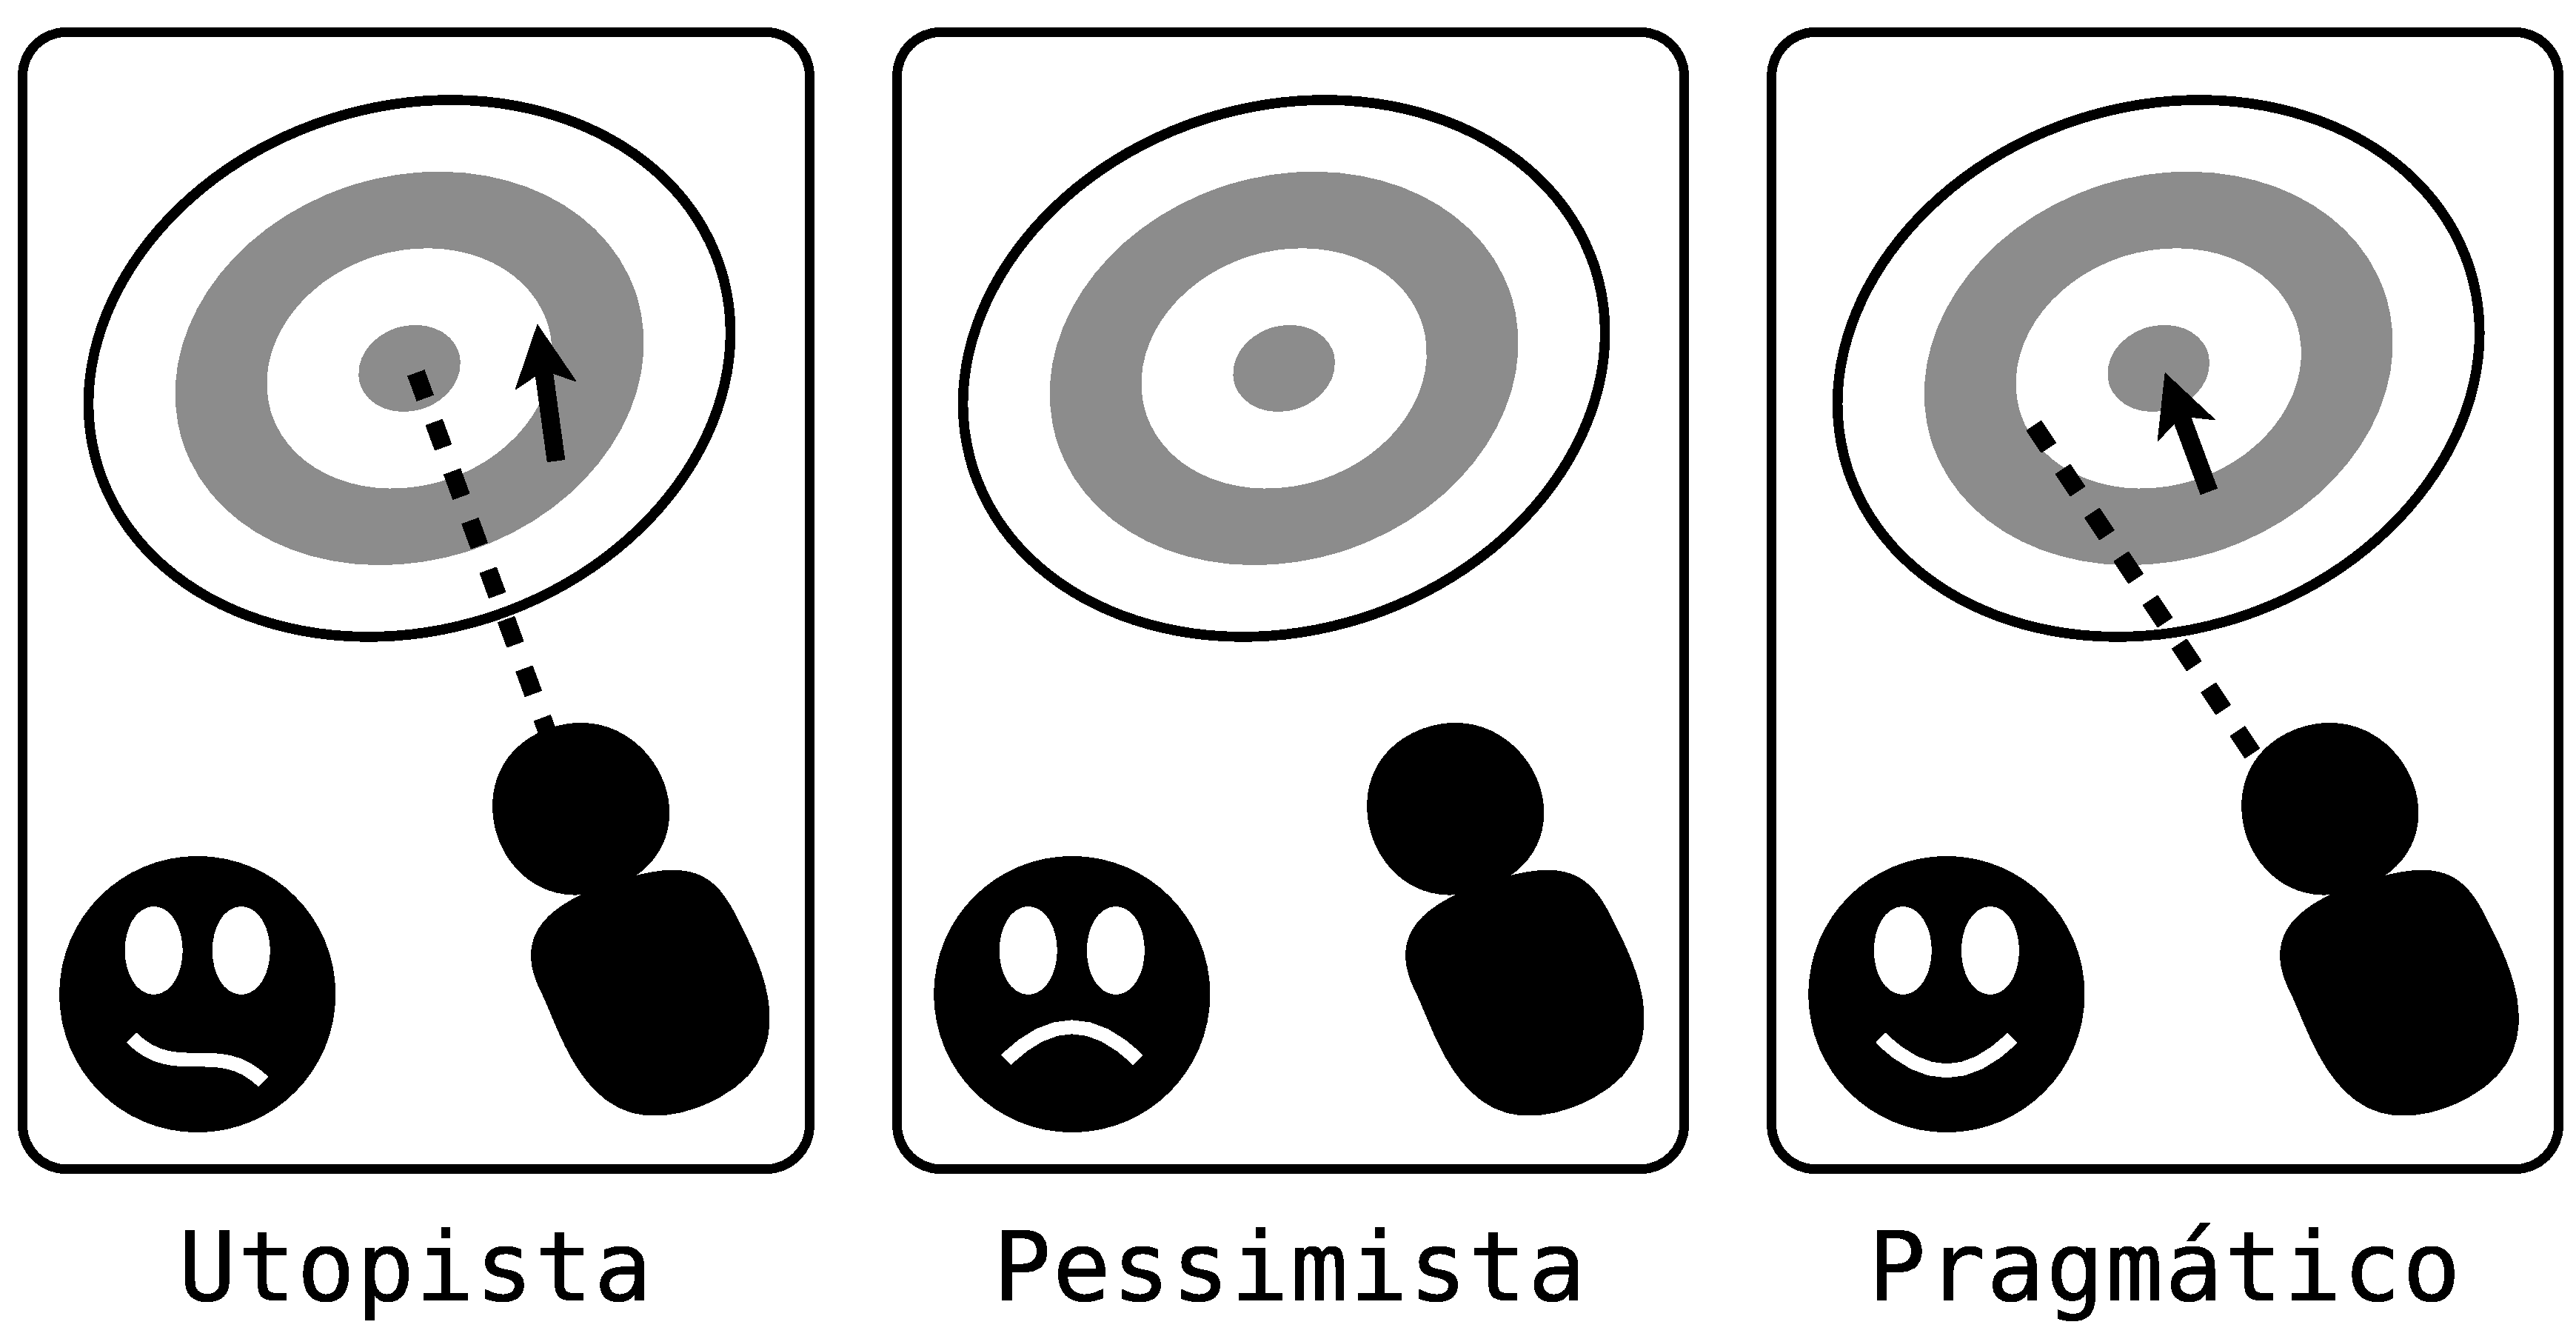
\includegraphics[width=0.7\textwidth]{chapters/cap-body-control/problema-generico-completo.eps}
\end{center}
\end{elaboracion}
\end{figure}


Mesmo que nestos casos poderíamos alegar que os problemas não são graves,
devemos prestar atenção que estes manifestam que a pessoa não tem conhecimento e domínio do seu corpo,
e isto pode impedir que a pessoa aprenda movimentos mais complexos,
pois ainda não tomou consciência da importância de conhecer seu próprio corpo para poder controlá-lo.
Nos casos anteriores é possível ter uma abordagem pragmática dos problemas.
Por exemplo:
\begin{description}
\item[Solução ao problema do movimento 1:] Se ao tentar em ir em linha reta, realizamos uma curva a esquerda,
em vez de tentar ir em linha reta, podemos tentar ter uma pequena desviação à direita,
ate que consigamos conferir que finalmente realizamos uma linha reta.
\item[Solução ao problema do movimento 2:] Se ao realizar um movimento de frente traz no samba de gafieira,
não podemos evitar colocar o pé direito atrás,
como quando dançamos forró; 
então uma solução seria deixar de tentar colocar ambos pés juntos,
e em cambio ordenar a nosso corpo colocar o pé direito ligeiramente adiantado,
ate perceber que na realidade colocamos os pés juntos.
\end{description} 


\begin{figure}[!ht]
\begin{elaboracion}{Ah\'i viene Mart\'in Corona (1952)}

A modo de anedota é interessante mencionar que esse desvio natural,
que as pessoas temos no nosso senso espacial, 
é muito conhecido desde antanho por pessoas pragmáticas;
por exemplo, podemos ver uma referencia a isto no filme ``Ahí viene Martín Corona'' (1952),
ambientado em México na época de vaqueiros, quatreiros e pistolas,
quando a personagem ``Piporro'', amigo da família de ``Martín'', 
apos perseguir e dar castigo aos assassinos dos pais do Martín, ainda criança, 
ensina a este a disparar.
O seguinte dialogo acontece aproximadamente aos 4 min. 15 seg. iniciado o filme.
\begin{description}
\item[Piporro:] 
Para ``pegar-lhe''\footnote{\label{foot:pegarle}Pegar-lhe: Atirar e atingir.} ao centro de um relógio, 
tem que lhe apontar abaxinho do 6. %\footnote{\label{foot:abaixinho}Abaixinho: Diminutivo de abaixo.}
Agora que se quer ``pegar-lhe''\footref{foot:pegarle} a um criminal na 
``mera''\footnote{\label{foot:mera}Mera | Mero: Palavra que serve para realçar; exatamente na.} frente, não tem perca,
aponta-lhe ao ``ocico''\footnote{\label{foot:ocico}Ocico: Focinho.}.
Agora que se trata-se de ``pegar-lhe''\footref{foot:pegarle} a 
um ``pelao''\footnote{\label{foot:pelao}Pelao: Pessoa grosseira, vulgar e inculta.} 
``fachoso''\footnote{\label{foot:fachoso}Fachoso: Desleixado excêntrico e extravagante.} no ``mero''\footref{foot:mera} coração,
escuta, segue este conselho, aponta-lhe ao umbigo.

\item[Martin:] Ao umbigo?

\item[Piporro:] Ao ``mero''\footref{foot:mera} umbigo! você que lhe aponta ai, ele que cai, sem dizer ai.
\end{description}
\end{elaboracion}
\end{figure}

